\documentclass{sigchi-ext}
% Please be sure that you have the dependencies (i.e., additional
% LaTeX packages) to compile this example.
\usepackage[T1]{fontenc}
\usepackage{textcomp}
\usepackage[scaled=.92]{helvet} % for proper fonts
\usepackage{graphicx} % for EPS use the graphics package instead
\usepackage{balance}  % for useful for balancing the last columns
\usepackage{booktabs} % for pretty table rules
\usepackage{ccicons}  % for Creative Commons citation icons
\usepackage{ragged2e} % for tighter hyphenation

% \usepackage{marginnote} \usepackage[shortlabels]{enumitem}
% \usepackage{paralist}

%% EXAMPLE BEGIN -- HOW TO OVERRIDE THE DEFAULT COPYRIGHT STRIP --
% \copyrightinfo{Permission to make digital or hard copies of all or
% part of this work for personal or classroom use is granted without
% fee provided that copies are not made or distributed for profit or
% commercial advantage and that copies bear this notice and the full
% citation on the first page. Copyrights for components of this work
% owned by others than ACM must be honored. Abstracting with credit is
% permitted. To copy otherwise, or republish, to post on servers or to
% redistribute to lists, requires prior specific permission and/or a
% fee. Request permissions from permissions@acm.org.\\
% {\emph{CHI'14}}, April 26--May 1, 2014, Toronto, Canada. \\
% Copyright \copyright~2014 ACM ISBN/14/04...\$15.00. \\
% DOI string from ACM form confirmation}
%% EXAMPLE END

\title{Wikidata Human Gender Index}

\numberofauthors{4}
% Notice how author names are alternately typesetted to appear ordered
% in 2-column format; i.e., the first 4 autors on the first column and
% the other 4 auhors on the second column. Actually, it's up to you to
% strictly adhere to this author notation.
\author{%
  \alignauthor{%
    \textbf{First Author}\\
    \affaddr{University of Author} \\
    \affaddr{Authortown, CA 94022, USA} \\
    \affaddr{author1@anotherco.edu} }\alignauthor{%
    \textbf{Fifth Author}\\
    \affaddr{YetAuthorCo, Inc.}\\
    \affaddr{Authortown, BC V6M 22P Canada}\\
    \email{author5@anotherco.com} } \vfil \alignauthor{%
    \textbf{Second Author}\\
    \affaddr{VP, Authoring}\\
    \affaddr{Authorship Holdings, Ltd.}\\
    \affaddr{Awdur SA22 8PP, UK}\\
    \email{author2@author.ac.uk} }\alignauthor{%
    \textbf{Sixth Author}\\
    \affaddr{Universit\'e de Auteur-Sud}\\
    \affaddr{40222 Auteur France}\\
    \email{author6@author.fr} } \vfil \alignauthor{%
    }
    }	

% Paper metadata (use plain text, for PDF inclusion and later
% re-using, if desired)
\def\plaintitle{SIGCHI Extended Abstracts Sample File: Note Initial
  Caps} \def\plainauthor{First Author, Second Author, Third Author,
  Fourth Author, Fifth Author, Sixth Author}
\def\plainkeywords{Authors' choice; of terms; separated; by
  semicolons; include commas, within terms only; required.}
\def\plaingeneralterms{Documentation, Standardization}

%% Set up our PDF with metadata
\hypersetup{%
  pdftitle={\plaintitle}, pdfauthor={\plainauthor},
  pdfkeywords={\plainkeywords}, }

% \reversemarginpar%

\begin{document}

\maketitle

% Uncomment to disable hyphenation (not recommended)
% https://twitter.com/anjirokhan/status/546046683331973120
\RaggedRight{} 

% Do not change the page size or page settings.
\begin{abstract}
  UPDATED---\today. This sample paper describes the formatting
  requirements for SIGCHI Extended Abstract Format, and this sample
  file offers recommendations on writing for the worldwide SIGCHI
  readership. Please review this document even if you have submitted
  to SIGCHI conferences before, as some format details have changed
  relative to previous years. Abstracts should be about 150
  words. Required.
\end{abstract}

\keywords{\plainkeywords}

\category{H.5.m}{Information interfaces and presentation (e.g.,
  HCI)}{Miscellaneous}\category{See}{\url{http://acm.org/about/class/1998/}}{for
  full list of ACM classifiers. This section is required.}

\section{Introduction}
Problematize introduction and make obvious need.

Landscape of ways in which Wikipedia shows bias, and Landscape of biases.

Our first observation is from September 17th 2014, and latest is January 3rd 2016. Although our dataset is now updated weekly following the official data dumps, automation was not completed until June 28th 2015, and so there is a window missing from October 2014 to June 2015. 

Albeit with caveats and huge biases, if the data is to believed, affords us an unprecedented look at gender representation on a time and geographic scale not possible before.

Introduce the dataset, and it's potential applications.	
\section{Dataset Details}

The Data is collected by (I'm sure I've written this somewhere already).


How to use the data.

Where is it located.
What types of files.
How is it updated.
How can they be used. 

Show demonstrations of graphs from the website.

There is little cleaning done. More on this later.

\section{Longitudinal Data}
Total humans in Wikidata increased from 5,869,606 to 6,999,542, and shows linear, unconstrained growth.
\begin{figure}
\label{fig:totalhumans}
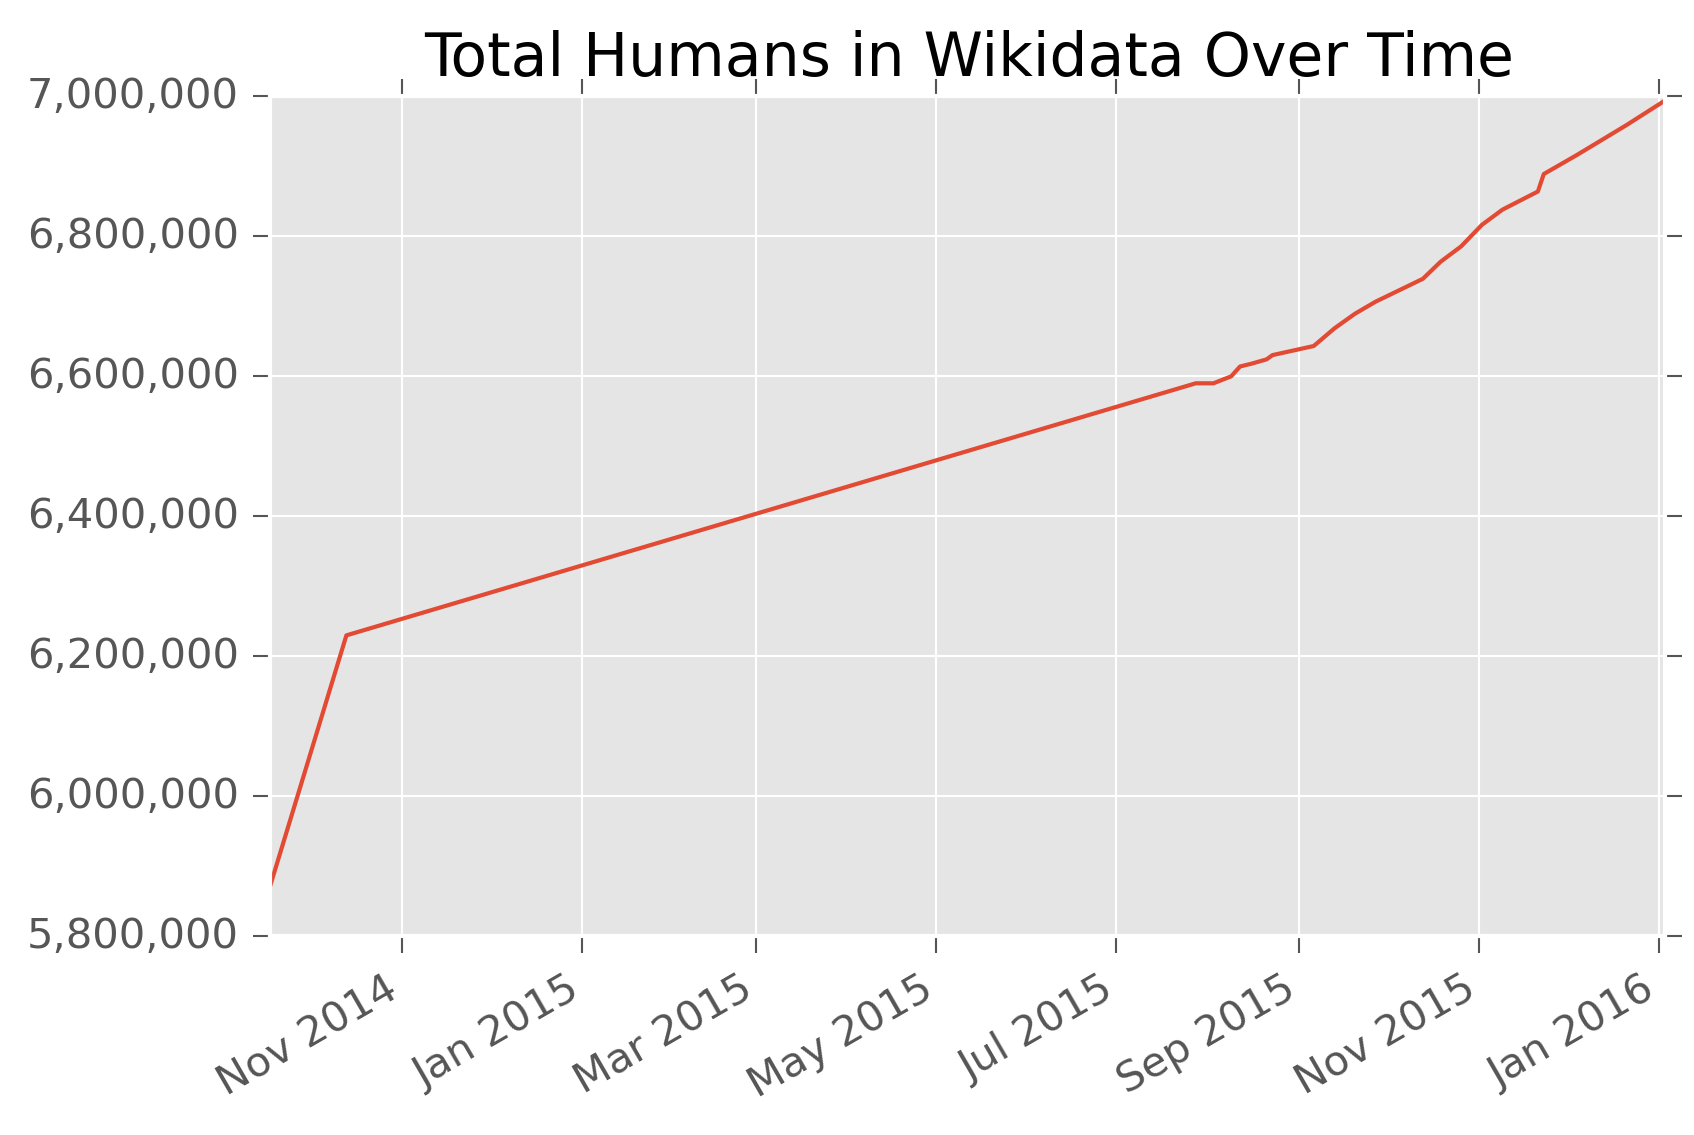
\includegraphics[scale=0.6]{figures/totalhumans.png} 
\caption{Total number of humans found in Wikidata at each snapshot period.}
\end{figure}

We should also be curious to the data quality of the increasing humans. One way to think about this is about the how much data is accompanying these human entries. We looked at the properties citizenship, place of birth, and ethnic group which will help us best geographically place a human. Another mark of quality is whether a human in Wikidata has an entry in a Wikipedia - a ``sitelink" in Wikidata vocabulary. \ref{fig:accompanying} shows the rate of accompanying properties, at the earliest and latest snapshots from 2014 and 2016 respectively. The statistics show that data quality has been increasing uniformly over time. The number of humans with \textit{gender} data increased by over 1\%, closer to complete coverage. Likewise \textit{citizenship} data increased by 15\% , \textit{place of birth} by 6\%  , and \textit{ethnic group} almost doubled \ref{table:accompanying}. Curiously the rate of humans having sitelinks decreased slightly. 

A Wikidata human without a Wikipedia article is know as a ``structural item"; for instance a Monarch without a Wikipedia article, but is a needed link in a family tree. With the view that a structural item is an artefact from humans paying attention to Wikidata's structure, the decrease in sitelinked humans can also be seen as a rise in data quality.

\begin{table}
\caption{Change in rates of human-accompanying properties}
\begin{tabular}{lrrrrr}
\toprule
snapshot &  gender &  citizenship &  place of birth &  ethnic group &  at least 1 site link \\
\midrule
2014-09-17 &  95.29\% &       42.82\% &          24.01\% &         0.31\% &                99.62\% \\
2016-01-03 &  96.54\% &       58.22\% &          30.51\% &         0.56\% &                98.15\% \\
\bottomrule
\end{tabular}

\label{table:accompanying}
\end{table}

\begin{figure}
\label{fig:accompanying}
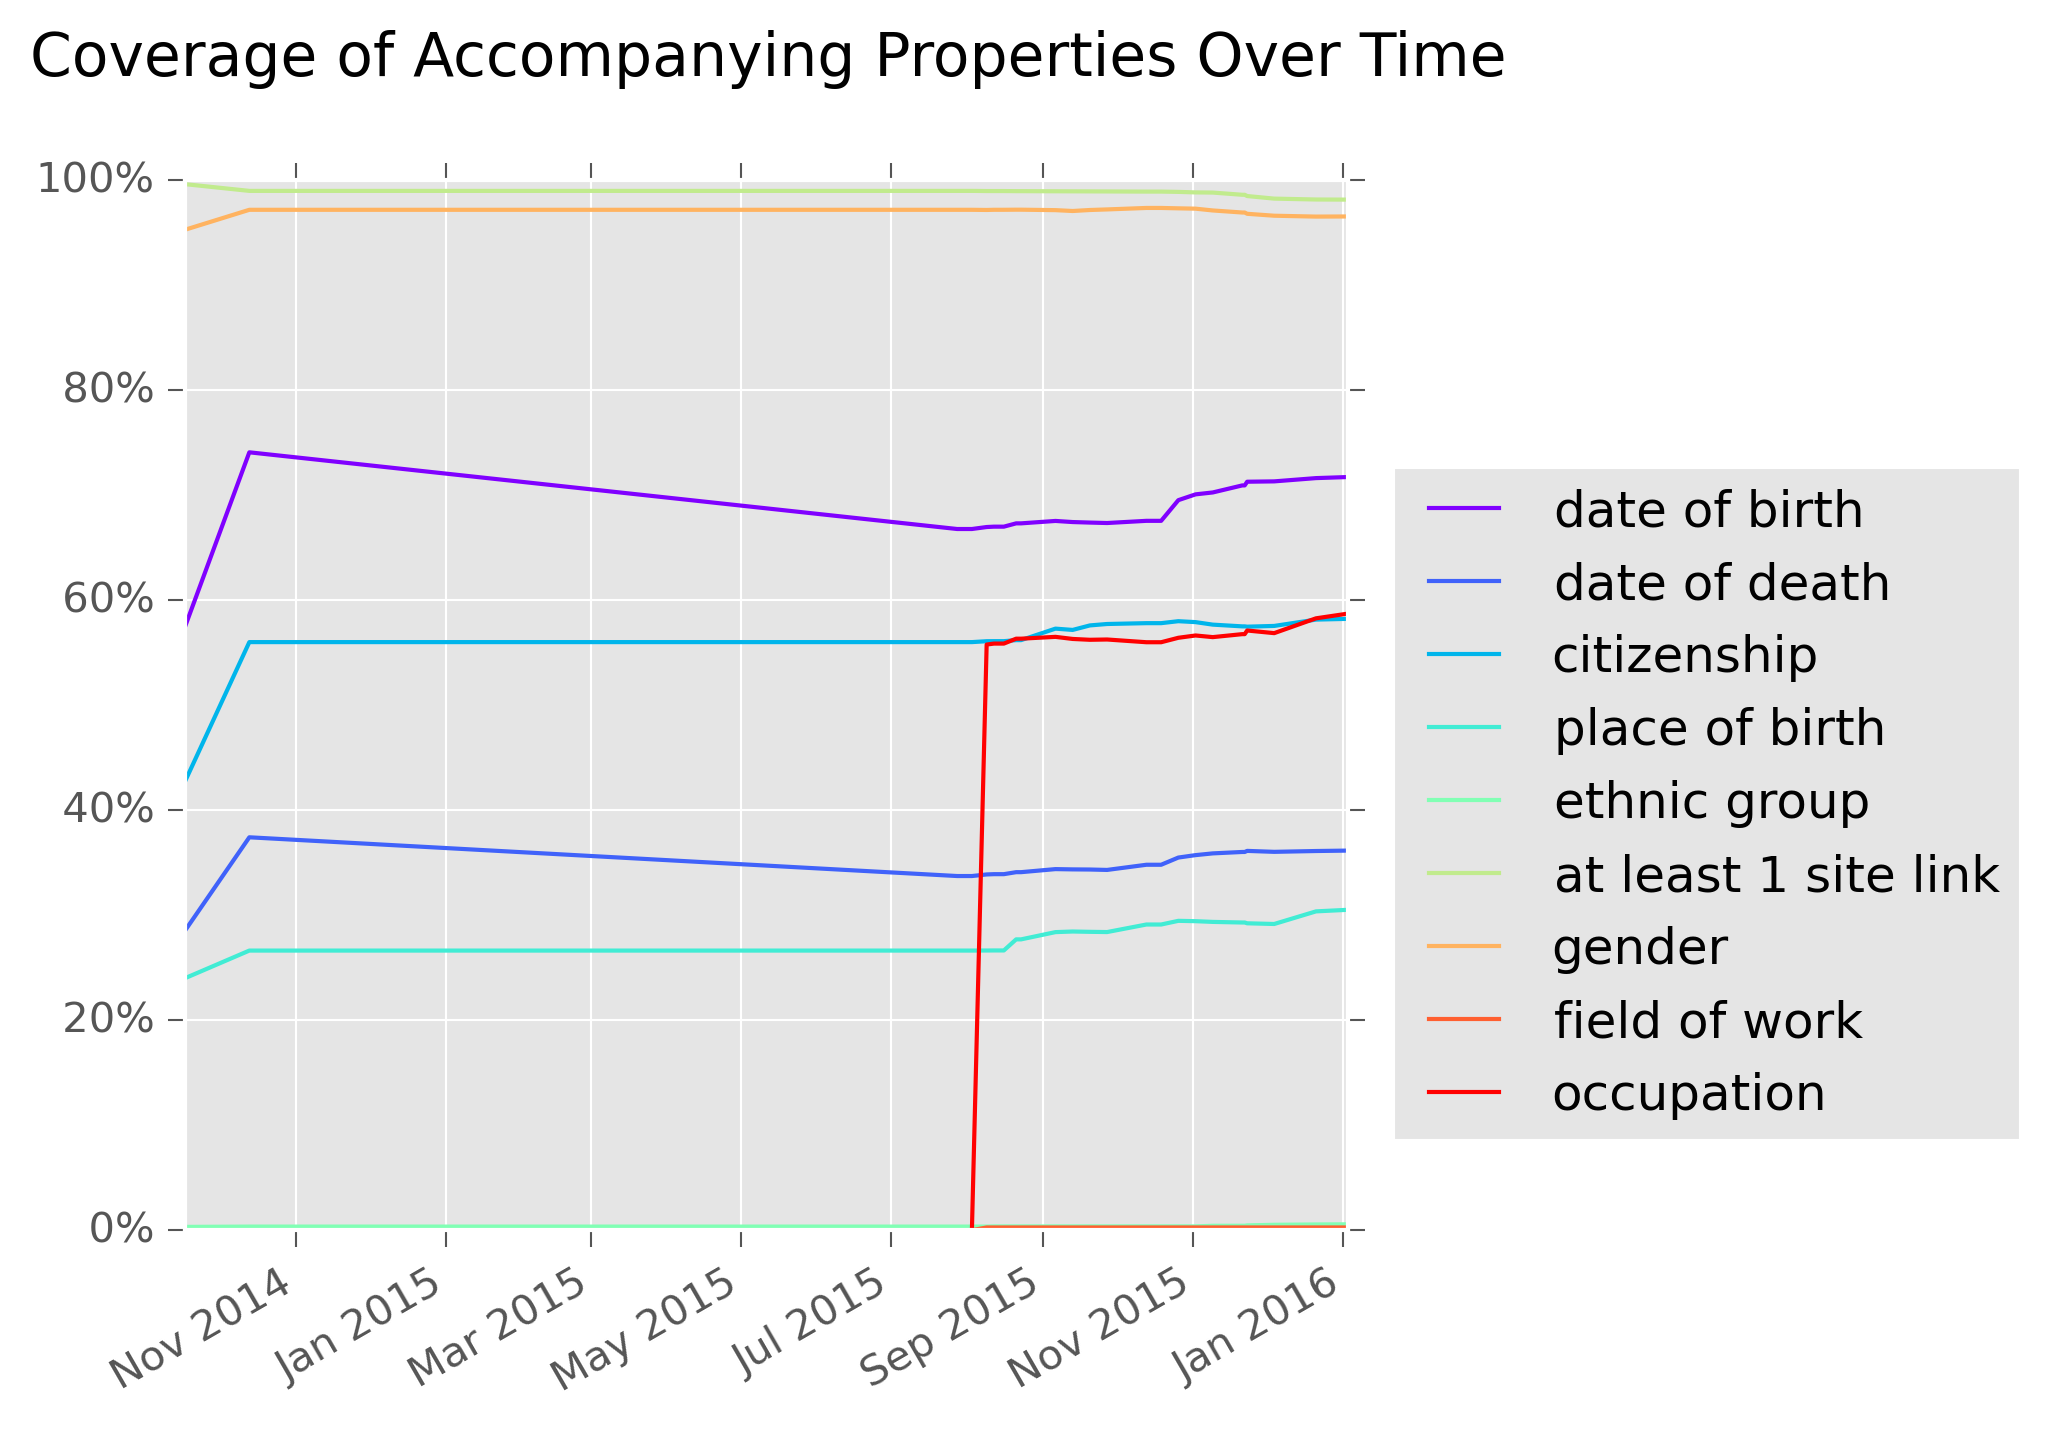
\includegraphics[scale=0.6]{figures/additionalprops.png} 
\caption{Trend of human-accompanying properties by snapshot.}
\end{figure}

Another important factor to note is that our dataset tries not to clean itself to fit any model. In fact the ``gender" property in Wikidata is actually labelled in English ``sex or gender" (no distinction), and not limited to any value. Over our time recording we found 36 values used for ``sex or gender", including ``male" and ``female", but extending to nonbinary genders ``transgender female", ``intersex", ``fa'afafine", ``transgender", ``Gender fluid",  ``genderqueer", ``kathoey", and ``queer". At times the other information is recorded such as ``gay", or ``homosexuality" and ``Alien" or "cheetah". And even what seem to be mistakes are left in such as  ``Solanum tuberosum", ``Messi", or ``sociologist".

Focusing on one of our motivations, monitoring the trend of gender representation, we inspect the rate at which women are recorded in Wikidata. \ref{fig:frb} shows the ratio of ``female" recorded humans versus all gendered biographies. Similarly to total biographies this measure is rising at a fairly linear rate of approximately 0.5\% per year. The final months on record show a slight decline which warrants further investigation. In fact being able to measure at a level where is precisely one of the points of having such a live-updating measure - to be able to detect trends as they happen, and perhaps relate them to community issues. 

\begin{figure}
\label{fig:frb}
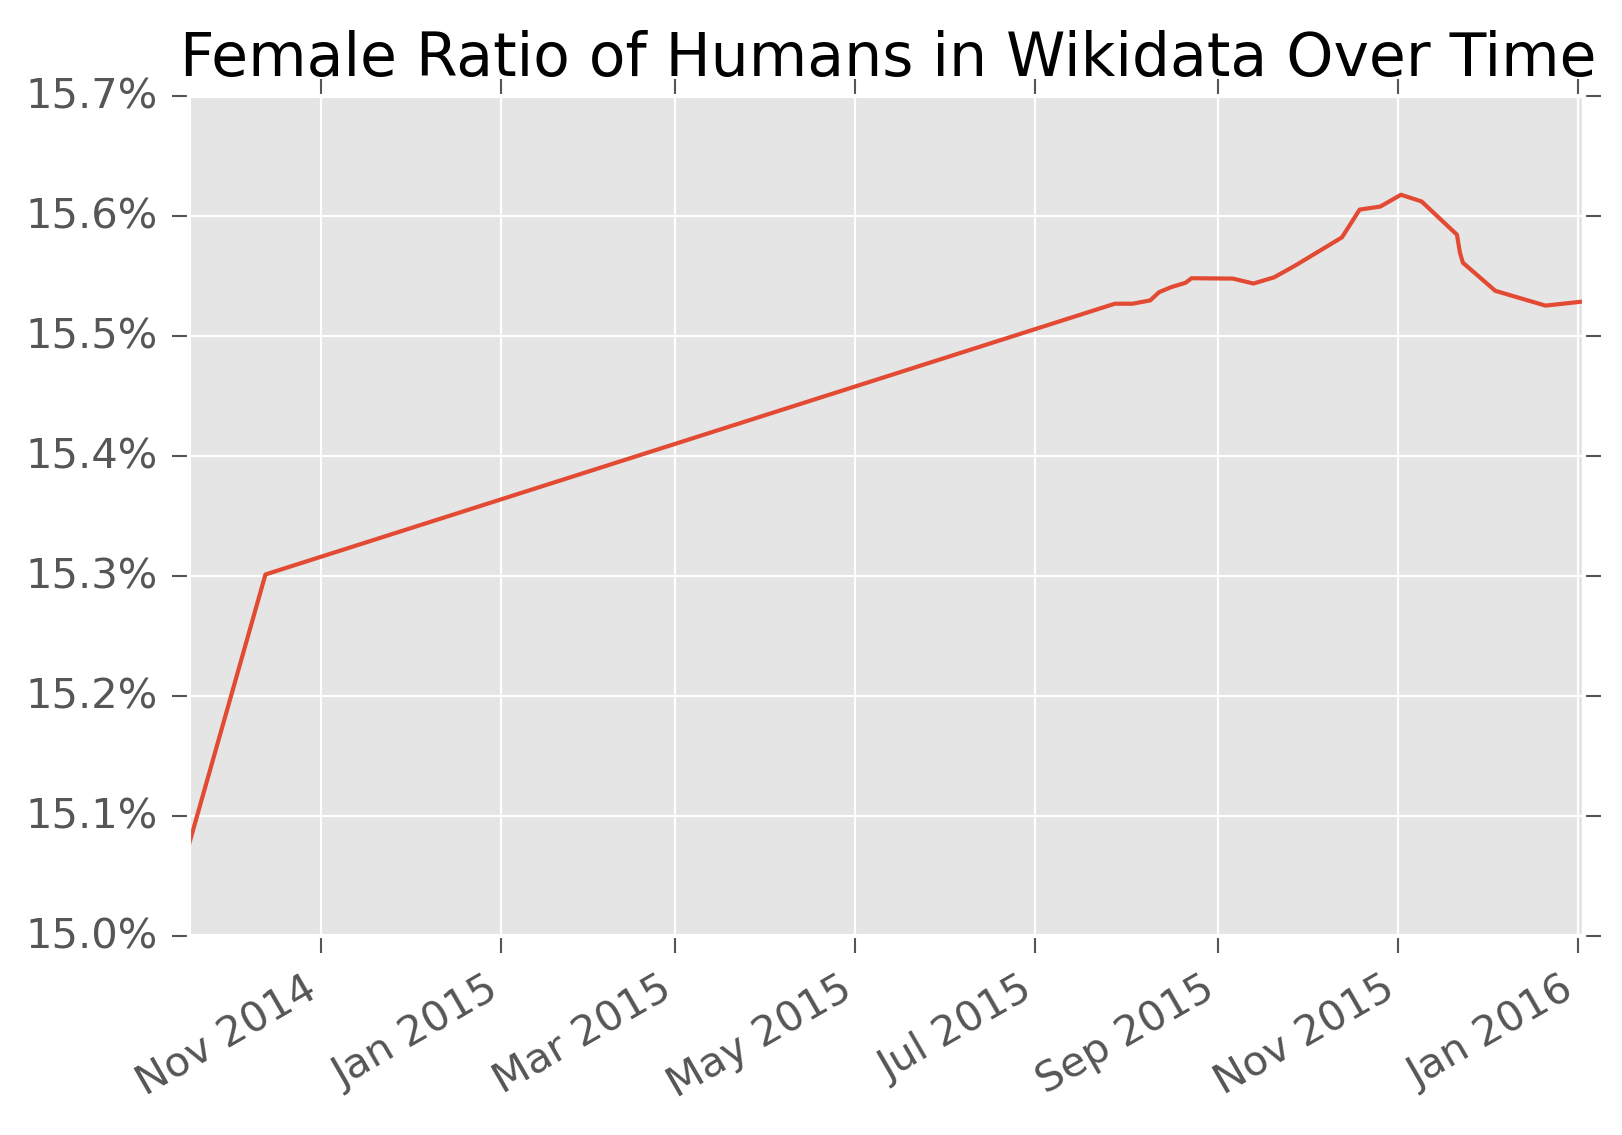
\includegraphics[scale=0.6]{figures/frbwikidata.png} 
\caption{Trend of human-accompanying properties by snapshot.}
\end{figure}

Another way in which Wikimedians can use the data is to look at trends specific to Wikipedia languages. It is easy to use the data to compile a top-10 list of Wikipedias whose female ratio of humans increased the most, see \ref{table:top10}. This measure does not explain whether women's representation in those languages increased because because editors took longer to record women's gender in Wikidata and were catching up in the observed period, or that these languages became more women-focused over the snapshotting period.

\begin{table}
\caption{Top 10 Wikis by increase in female ratio of humans from October 2014 to January 2016}
\label{table:top10}
\begin{tabular}{p{2cm}p{2cm}}
\toprule
{Wiki} &     Increase in female ratio of humans  \\
\midrule
Lithuanian      & 5.31\% \\
Japanese     & 4.76\% \\
Estonian      & 4.58\% \\
Slovenian      & 2.19\% \\
Tagalog      & 1.63\% \\
Korean      & 1.38\% \\
Finnish      & 1.33\% \\
Wikimedia Commons & 1.20\% \\
Farsi      & 1.17\% \\
Hebrew      & 1.17\% \\
\bottomrule
\end{tabular}


\end{table}

\section{Validation}
We validated out data by comparing it against 3 exogenous measures. Wikidata date of birth frequency versus historical world population trends, Wikidata gender by country  versus external by-country gender-disparity indexes, and Wikidata occupation gender versus United States Bureau of Labour Statistics occupation gender.

\subsection{World Population}

\subsection{External Indices}
Calibrated start dates were each 1900 or 1910 - a good sign. Over time the the WHGI-county is become more correlated to major external gender-disparity indexes \ref{table:scores}. In context with the fact that data quality is rising, this can be taken to mean that as Wikidata becomes more complete it is modelling the real world more. 

 \begin{table}
\caption{WHGI-country correlation to external indices. Correlation is the Spearman $\rho$, and signficances are *p<0.05, **p<0.01}
\label{table:scores}
\begin{tabular}{lrrrr}
\toprule
snapshot &  GEI &  SIGI &  GGGI &  GDI  \\
\midrule
2014-09-17 &  0.417** &       0.338** &          0.310* &         0.278**  \\
2016-01-03 &  0.457** &       0.402** &          0.386** &         0.299**  \\
\bottomrule
\end{tabular}
\end{table}


\section{Potential Application}
Open Knowledge Foundation founder Rufus Pollock once said ``The best thing to do with your data will be thought of by someone else.”

FRB/wikisize. Is it data completeness or feminist-focus?


Use for determining women's notability for historical events.

Linking with VIAF. 

Comparing language's inherent gender bias to shown.

Wikimedian communities can use this an introspective watch.

Useful in all the same ways that external indices like the UNDP are too.

% \bibliographystyle{ACM-Reference-Format-Journals}
\bibliographystyle{SIGCHI-Reference-Format}
% \bibliographystyle{acm}
\bibliography{sample}

\end{document}

%%% Local Variables:
%%% mode: latex
%%% TeX-master: t
%%% End:
